\documentclass[11pt,a4paper]{article}
\usepackage{amsmath}
\usepackage{amssymb}
\usepackage{graphicx}
\usepackage{verbatim}
\begin{document}
\noindent
Martin Lundfall, Henri Bunting, Malte Siemers, Patrik Bey
\begin{centering}
  \section*{Exercise sheet 09 - Machine Intelligence I}
  \end{centering}
\section*{9.1}
The primal problem for C-SVMs is solved by using the Karush-Kuhn-Tucker conditions, a generalization of Lagrange multipliers. We aim to minimize the following equation:
\begin{equation}
  L_{(w, b, \{\lambda_\alpha\})} = f_0(w, b) + \sum_{\alpha=1}^p \lambda_\alpha f_\alpha(x)
\end{equation}
Where $f_0$ is the function to be minimized, in our case:
\begin{equation}
f(w,b) = \frac{||w||^2}{2} + \frac{C}{p}\sum_{\alpha=1}^p \varphi_\alpha
\end{equation}
 and $f_k$ are the inequality constraints, in our case:
\begin{equation}
f_\alpha(w, b) = (1 - \varphi_\alpha) - y_T (w^Tx + b)
\end{equation}
\begin{equation}
f_\alpha(w, b) = - \varphi_\alpha
\end{equation}
We minimize the KKT equation first with respect to $w$. Note that the slack variables $\varphi_\alpha$ are independent of $w$. This results in:
\begin{equation}
w = \sum_{\alpha=1}^p \lambda_\alpha y_T^{(\alpha)}x^{(\alpha)}
\end{equation}
Then minimizing with respect to $b$ we get the following constraint on $\lambda_\alpha$:
\begin{equation}
0 = \sum_{\alpha=1}^p \lambda_\alpha y_T^{(\alpha)}
\end{equation}
Putting these results back into the KKT equation, we attain:
\begin{equation}
L_{(x_k, \{\lambda_k\})} = \frac{1}{2} \sum _{\alpha, \beta=1}^p\lambda_\alpha \lambda_\beta y_T^{(\alpha)}y_T^{(\beta)}(x^{(\alpha)})^Tx^{(\beta)}+\sum_{\alpha=1}^p\lambda_\alpha
\end{equation}
We clearly see that minimizing this equation corresponds to maximizing the expression given in the exercise. The upper bound of the $\lambda_\alpha$ variables is given by the duality of the problem.

\section*{9.3 - C-SVM with standard parameters}
\subsection*{a)}
We used the scikit.learn python package to create and train a C-SVM as can be seen in the file 9.3.py.
\subsection*{b)}
The mean error from the 0-1 loss function was 16.25\%
\subsection*{c)}
The plot of our classification with decision boundaries and false positives and false negatives highlighted:
\begin{figure}[h]
  \centering
  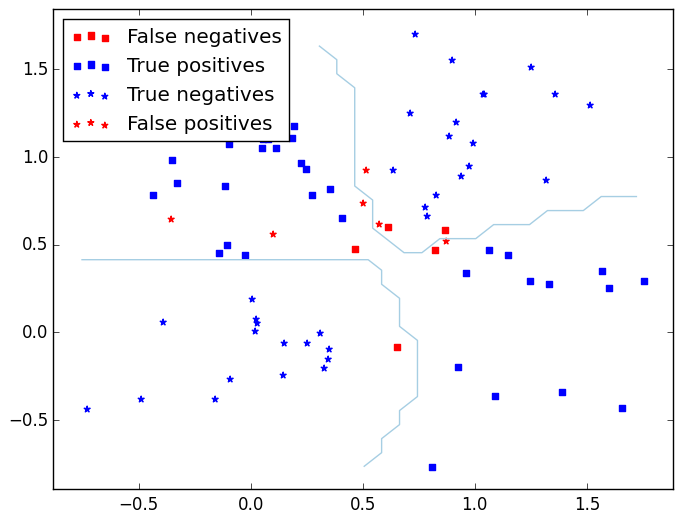
\includegraphics[width=\linewidth]{9_3.png}
\end{figure}

\section*{9.4 - Parameter Optimization}
\subsection*{(a)}
Following the procedure for grid search as described in the guide we performed leave-one-out cross validation (LOOCV) on the training data using the following parameter range:\\
$ \gamma = [2,2^{-1},2^{-3},2^{-5},2^{-7},2^{-9},2^{-13},2^{-15}] $, $ C = [2^{-5},2^{-3},2^{-1},2,2^{3},2^{5},2^{7},2^9]$\\
After that we refined the grid to:\\
$C = [2^{1.5},2^{1.75},2^2,2^{2.25},2^{2.5},2^{2.75},2^{3},2^{3.25},2^{3.5},2^{3.75},2^4,2^{4.25},2^{4.5}]$\\
$\gamma = [2^{-.5},2^{-.25},2^0,2^{.25},2^{.5},2^{.75},2^1,2^{1.25},2^{1.5},2^{1.75},2^2,2^{2.25},2^{2.5}]$\\
The parameter we obtained from the second grid search were $\gamma=0.8408$ and $C=16$. On the following pages the cross validation performance and the mean training classification for those parameters are shown, as well as the test data with the classification boundaries.
\subsection*{(c)}
The classification error was then 16.25\% and the CSVM used 42 supporting vectors.
\subsection*{(e)}
The classification error is the same as in our results with the standard parameters from the python package. The python package had to use 58 supporting vectors. Visually, the cross validated results show as well as the standard parameter results no signs of overfitting. We couldnt find a set of parameters, that significantly improved the results.

\begin{figure}[h]
	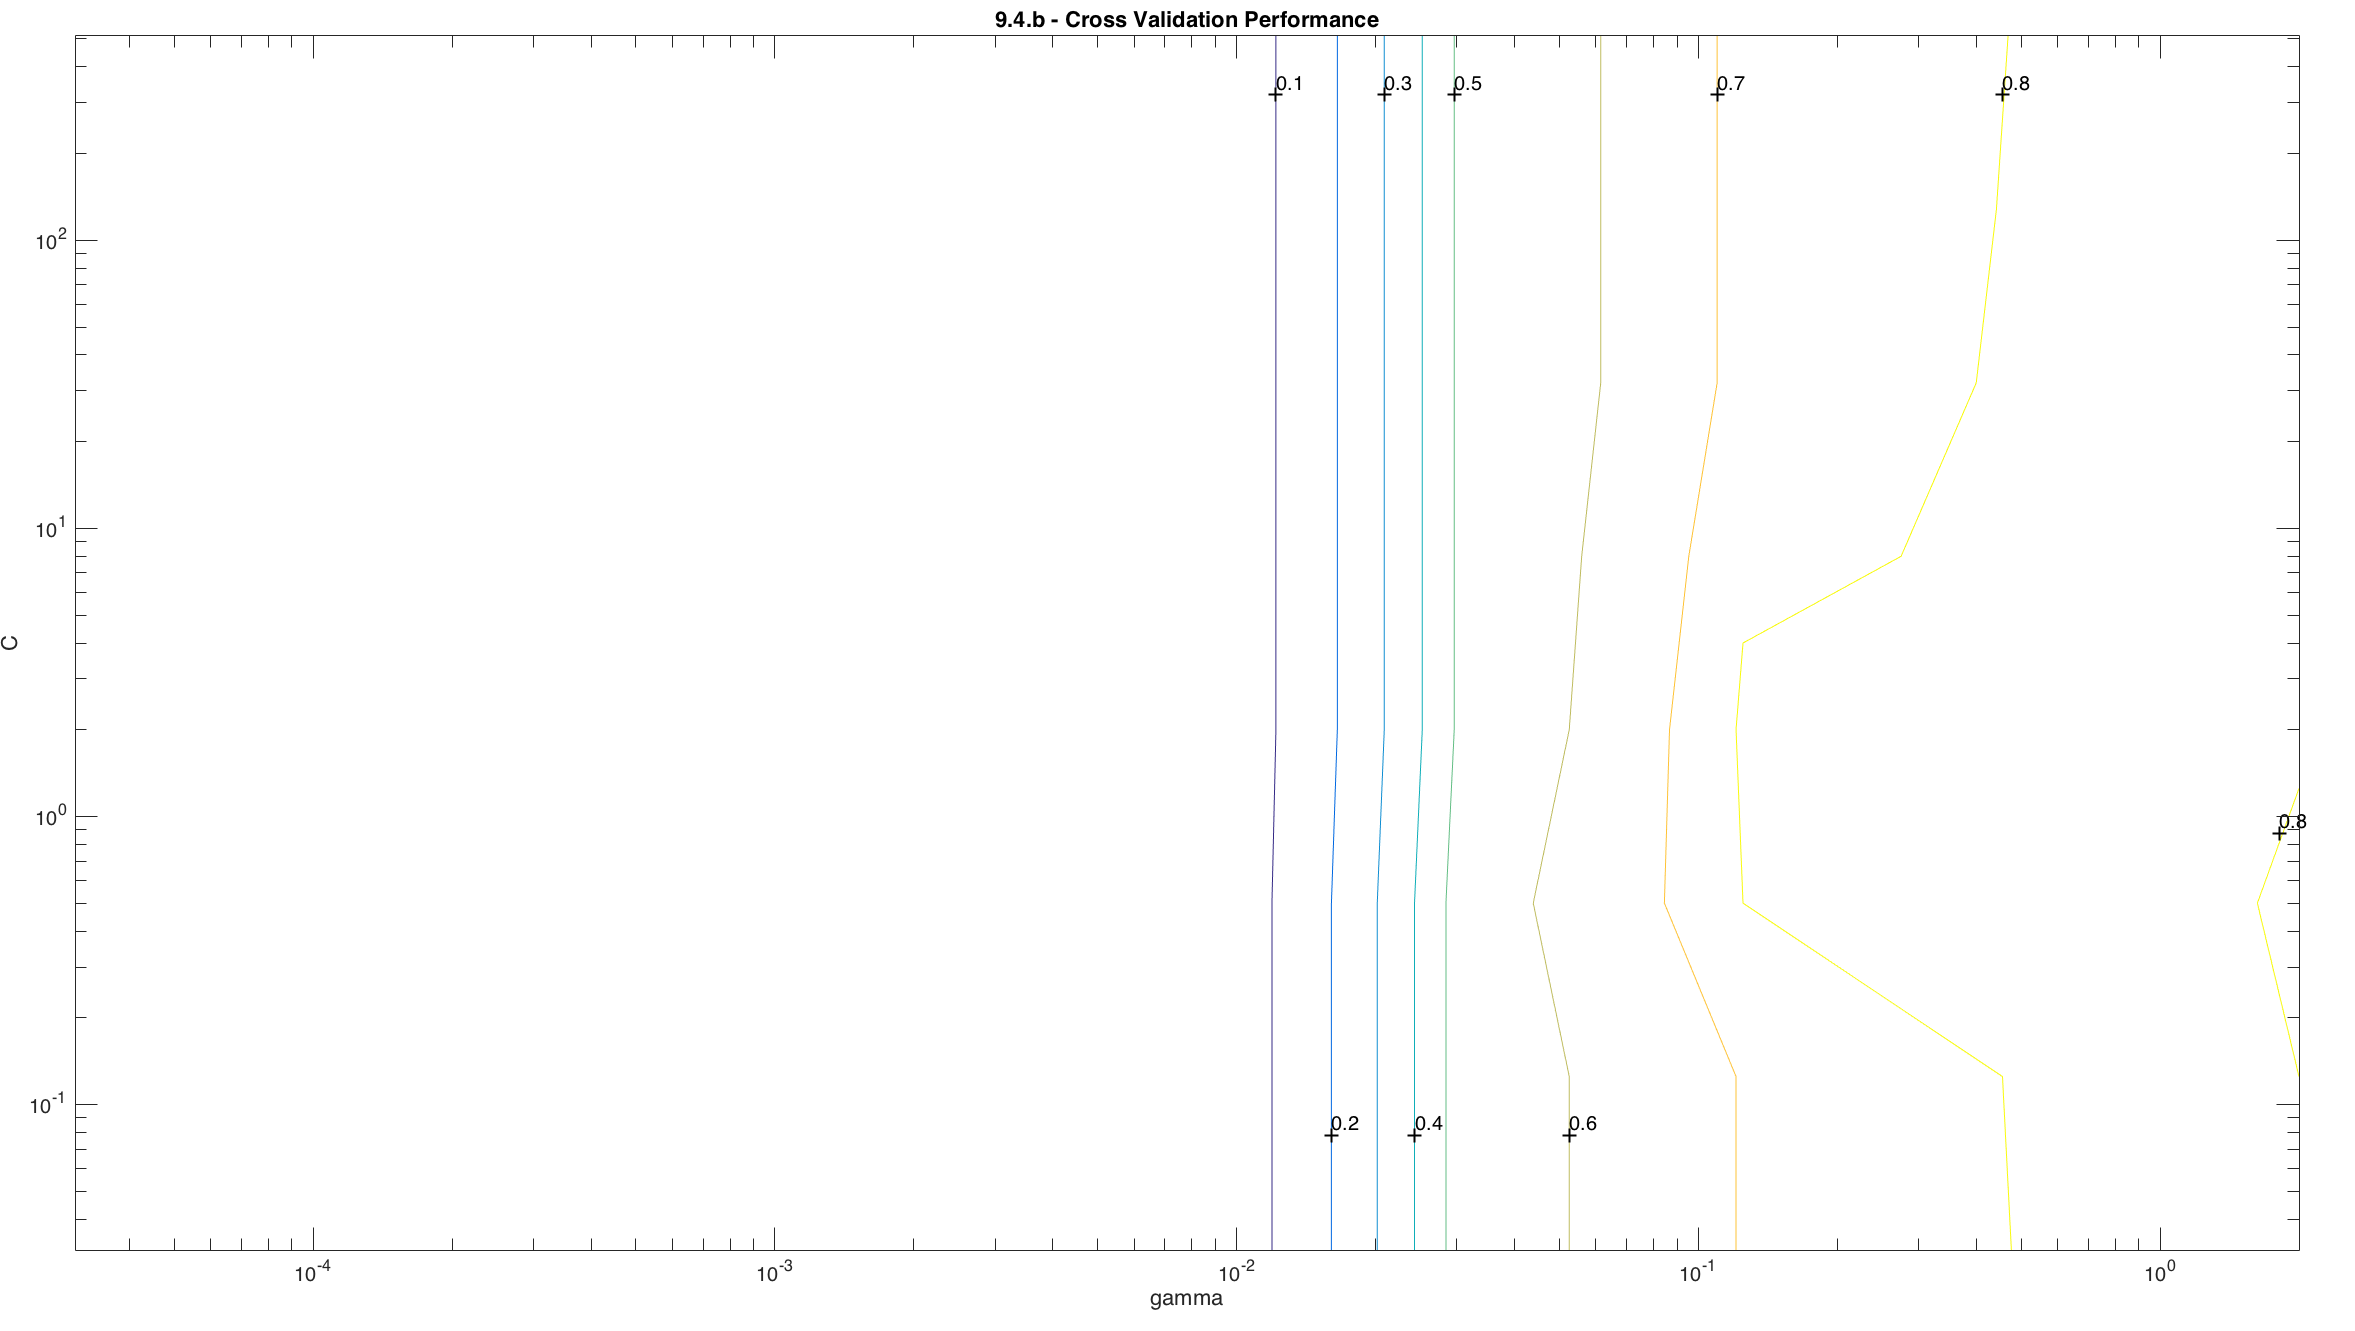
\includegraphics[angle=270,width=\textwidth]{94b_1.png}
	\centering
\end{figure}
\begin{figure}[h]
	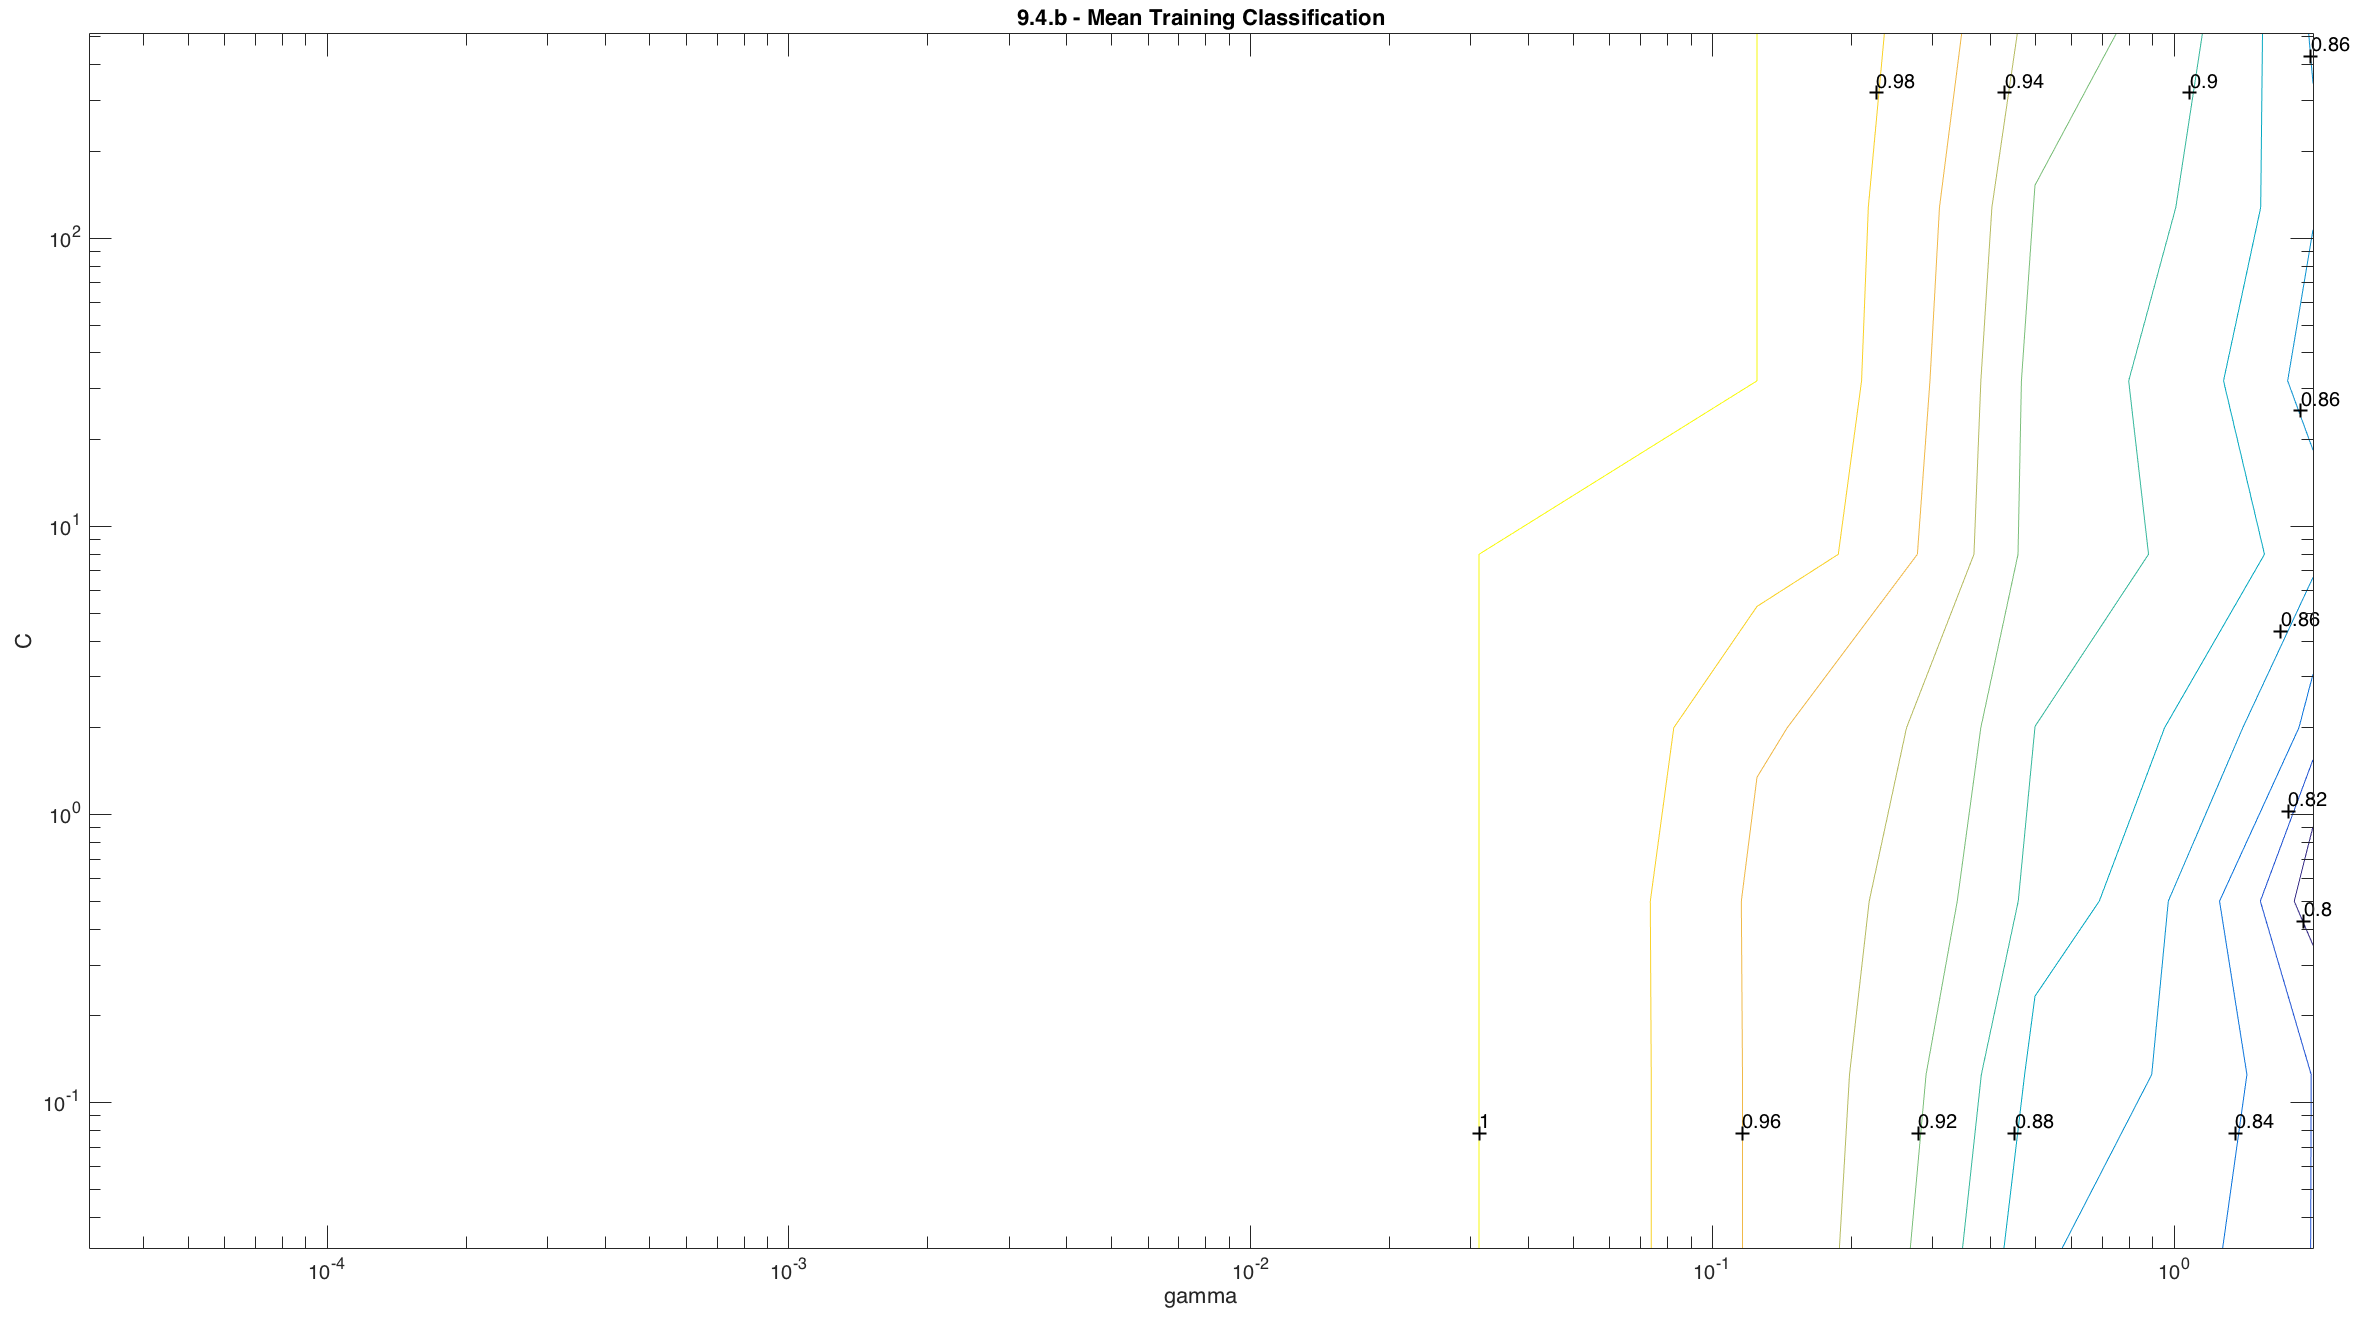
\includegraphics[angle=270,width=\textwidth]{94b_2.png}
	\centering
\end{figure}
\begin{figure}[h]
	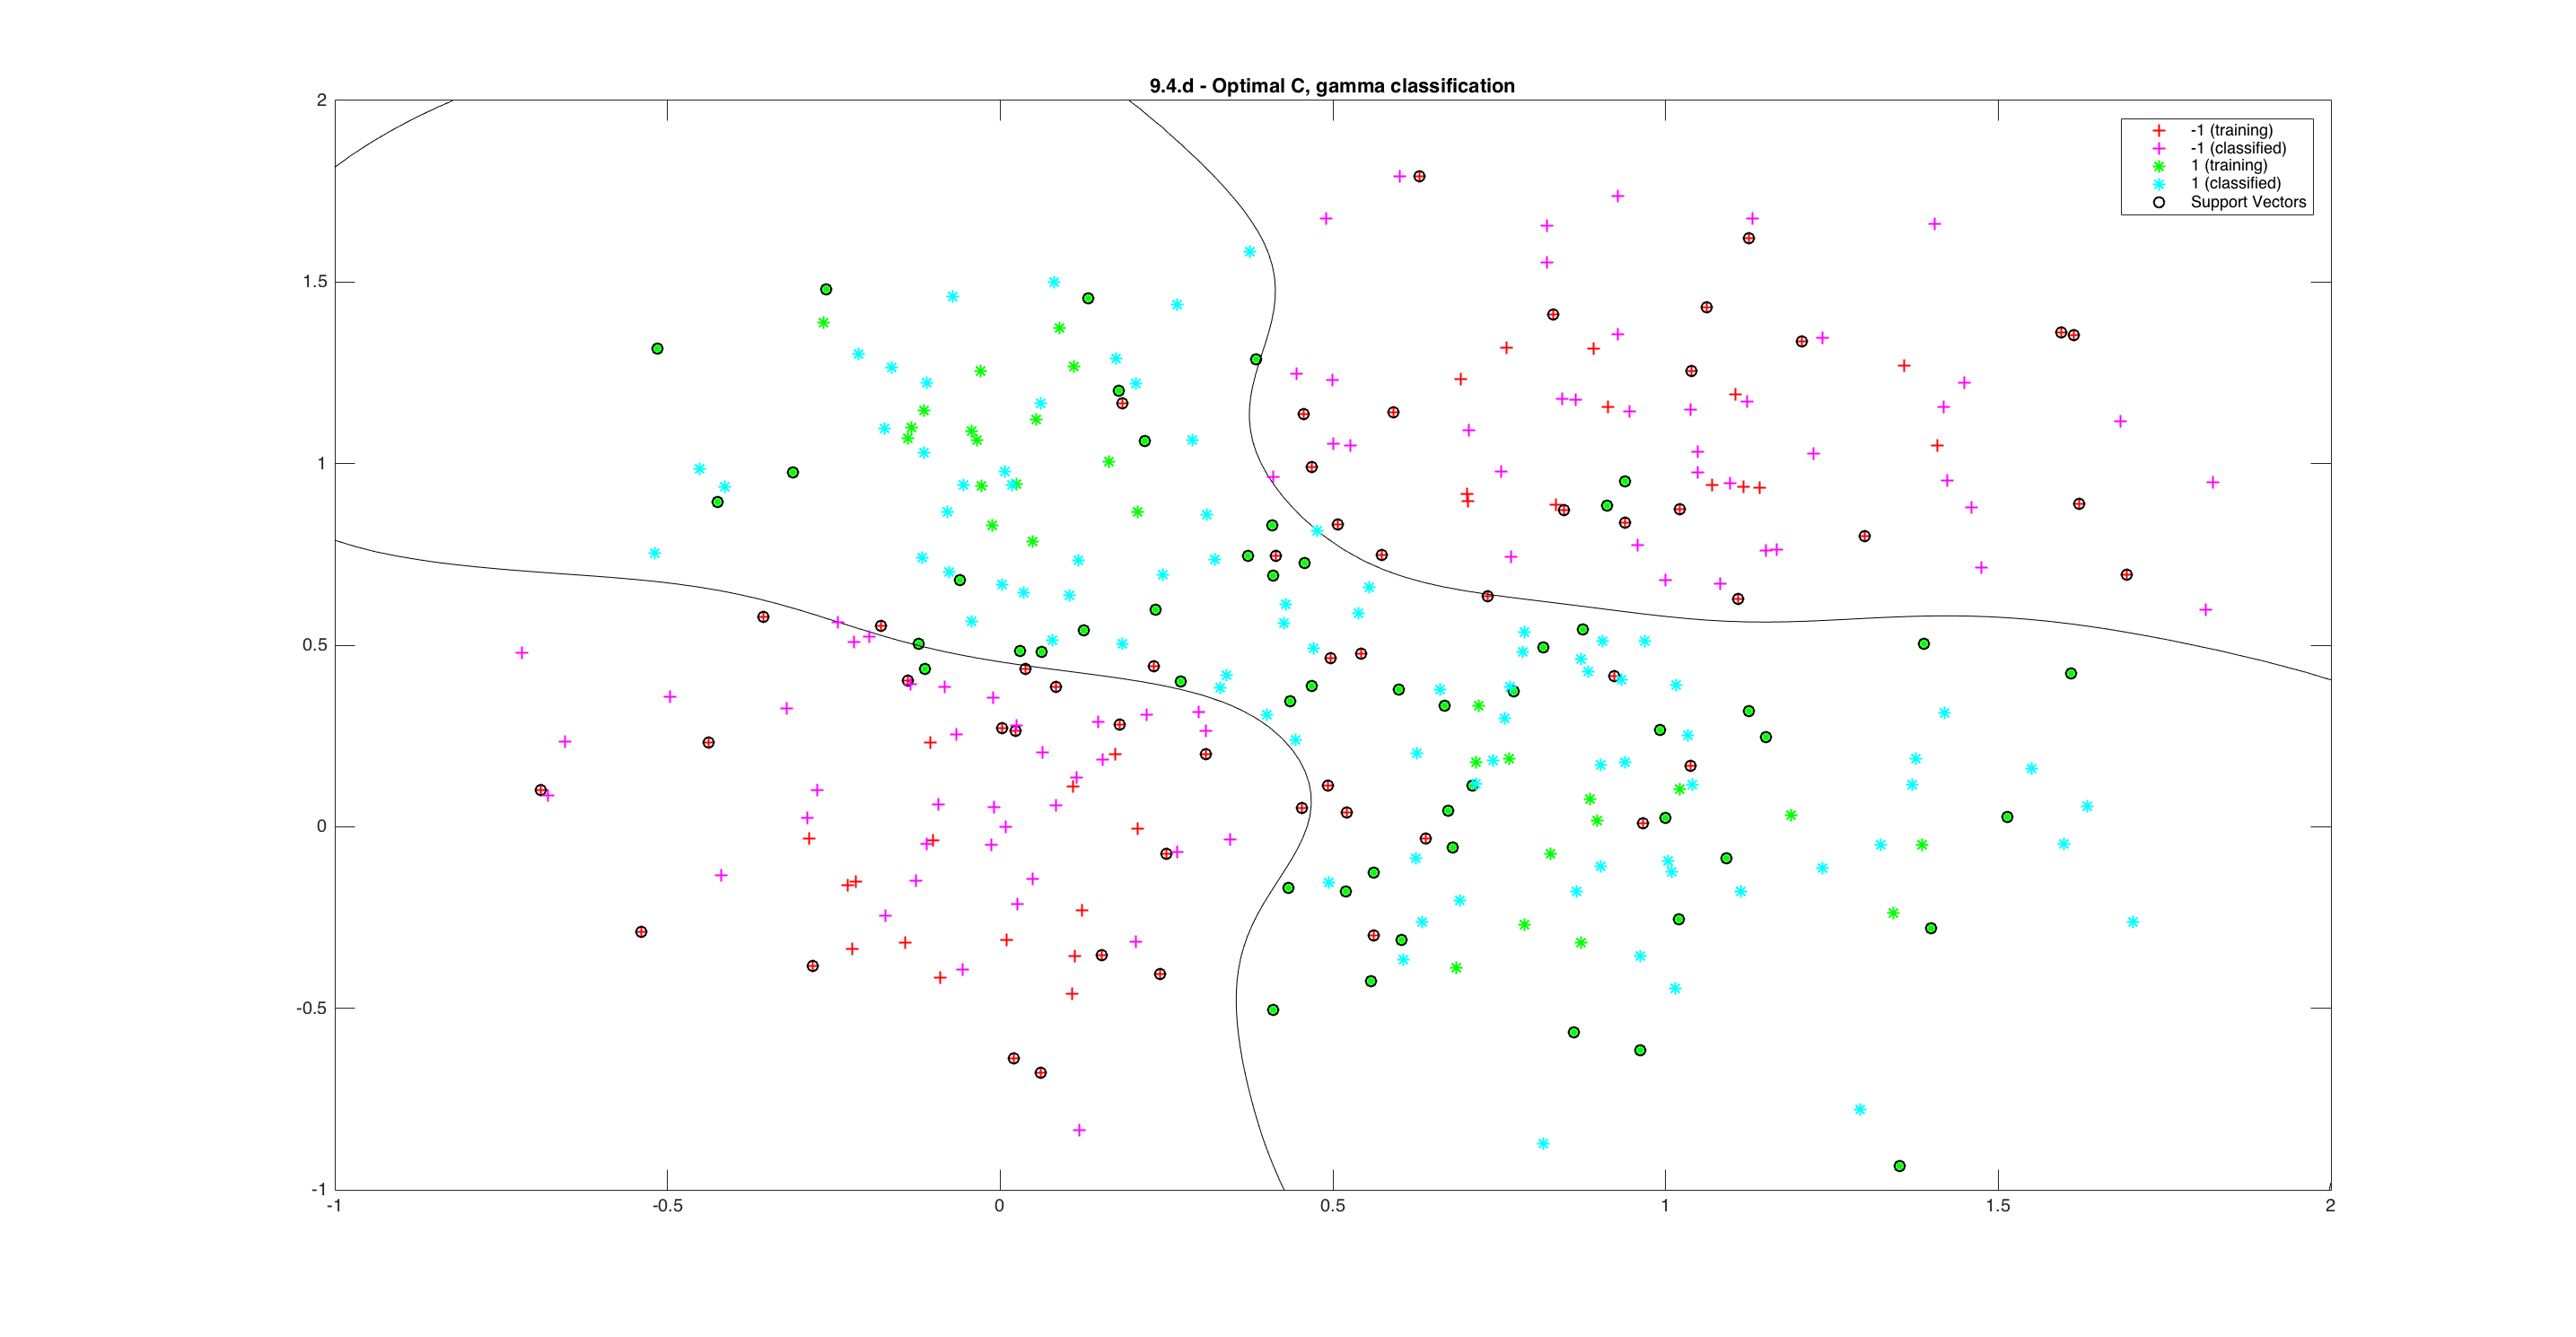
\includegraphics[angle=270,width=\linewidth]{94d.png}
	\centering
\end{figure}



\end{document}
